\chapter{Introduction}
\label{chp:introduction} 

\section{Motivation}
As of now the Mesh Potato has mainly been permanently deployed in small villages where the existing telecommunication systems are limited, non existent or too expensive. There are many scenarios where there is need for a solution that easily, and fast can provide people with telephone communication and Internet, both within a community, and with the outside world. These scenarios span from natural disasters, post-conflict situations, temporary refugee camps and IDP (internally displaced person) camps, to the use at festivals, when a mobile tower is non-functioning, or during a blackout. 

We hope to expand the potential of the Mesh Potato through our portable solution. We want to make it quick and easy to deploy, thus making it more useable in emergency situations. This does not only benefit the locals, but also makes the job easier for relief organizations. 
We want to provide communication where there are none,  and believe that with the “emergency box” time would be spared and lives can be saved.

An area that has not been fully explored is the use of Mesh Potatoes in emergency situations, like natural disasters, post-conflict situations, etc. Another area to be considered is the use of Mesh Potatoes in refugee camps, where many people quickly gather in a new location. In both situations, the need for communication is essential. Key factors of usage are quick roll-out and usability. Easy to use communication is extremely important in crisis situations, both communication within the camp and outgoing communication with the rest of the world. It is important that all affected have easy access to helpful information, as this could mean the difference between life and death in some situations. In refugee camps with thousands of people, registering and reuniting people can be a difficult task to solve. Communication technology, like the Mesh Potato, could be revolutionary in situations like these. 


\section{Problem Description}
As our main problem description shows, the initial approach on our thesis was to look info refugee camps and how the Mesh Potatoes could be utilized in these situations. We started contacting different Norwegian relief organizations, but found it hard to establish a good connection with any of them. We also saw that the field was enormous and to much for us to grasp with the limited amount of time that we had available. A deciding factor was also that we saw the need to visit a camp in order to understand how the refugee camps works, and what the need in forms of communication would be. Everyone that we were in contact with said that no two camps are the same or run in the same way. Also the camps are often run by the local government with help from the different relief organizations. Different countries have different laws and regulations, and these also have to be taken into consideration. Without being able to early in the process establish a cooperation with a relief organization, we decided to direct our focus in a slightly different direction. We therefore chose to look into the use of the Mesh Potato in different scenarios with the focus on quick roll-out and providing Internet.

Our main focus is to provide the people with Internet access, since it is crucial to have the possibility to communicate with the outside world during an emergency situation. In order to get Internet into the mesh network formed by the Mesh Potatoes, at least one of the Mesh Potatoes must be connected to Internet. Which type of access network that is available depends on the location. Some places there might exist stable landlines, other places not. Other options could then be to use satellite or cellular networks to provide the network with Internet.  

Our idea is to make an "emergency box" that consist of a Mesh Potato, a telephone, rechargeable battery, on/off switch and a solar panel to charge the battery. All this will be contained inside a robust and waterproof suitcase. All packed together and ready to go in any situation, at any time, anywhere in the world. 

Based on our motivation we researched and conducted a study in order to answer the following research questions: 

\begin{enumerate}
\item How are the Mesh Potatoes set up? 
\item How can an emergency box be developed? What components, set-ups and configurations are necessary?
\item What kind of up-links can we connect the Mesh Potato to? And how can this be done easily? 
\item How make the roll-out process as quick as possible? What measures can we do in advance to make it as easy and fast as possible to connect the emergency box to and internet connection?
\item In what kind of situations could there be a need for a portable emergency box? What are the need in the different situations?
\end{enumerate}


\section{Methodology}

Our studies have mainly consisted of researching, and looking into the technologies used by the Mesh Potato. Before we could start to answer the questions in our problem description, it was important to get knowledge and an understanding of the company, Village Telco, how it all started and what their vision is. We were in contact with some of the founders of Village Telco, which gave us a good insight to how it all started, how Village Telcos are created and what their motivation factors are. 

\begin{figure}[b]
  \centering
      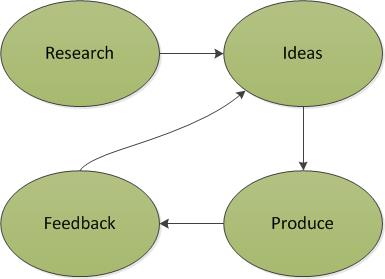
\includegraphics[width=0.6\textwidth]{metode.jpg}
  \caption [Methodology for making of the emergency box]{\textbf{Methodology for making of the emergency box.}}
  \label{fig:metode}
\end{figure}


In addition to having knowledge about the company and their vision, it is important to get an understanding of the technologies utilized. This enables the possibility to conduct further research and testing. After this theoretical learning process, we started looking into how Internet can be provided to mesh networks. 

The theoretical insight gave us ideas on how to expand the Mesh Potato's area of usage. We looked at specific scenarios in need of communication systems, and this brought forward the idea of creating an emergency box that could be applied for quick roll-out in different scenarios. The idea of the box is developed based on previous work conducted by others. This provided the foundation for our idea and our development of the box. The prototype was tested on x non-technical people. They provided us with valuable feedback, which lead to a new iteration in the making of the emergency box. 

We also tested and further developed the miscellaneous set-up descriptions provided by Village Telco. This was a big part of our assignment. Many of the existing descriptions are outdated and hard to understand, and also not valid for the second version of the Mesh Potato.



\section{Limitations}
Our main limitation was the amount of time we had available to finish our masters thesis, we only had 21 weeks at our disposal. When entering a new field it takes some time to understand the technology used. None of us have much experience with the different technologies used, and it took us some time to learn. Another limitation is money. We tried to get funding, from Engineers without Borders, to visit an area recently affected by a natural disaster. Unfortunately they had no funding available at the moment.


